\documentclass{beamer}

% xcolor and define colors -------------------------
\usepackage{xcolor}

% https://www.viget.com/articles/color-contrast/
\definecolor{purple}{HTML}{5601A4}
\definecolor{navy}{HTML}{0D3D56}
\definecolor{ruby}{HTML}{9a2515}
\definecolor{alice}{HTML}{107895}
\definecolor{daisy}{HTML}{EBC944}
\definecolor{coral}{HTML}{F26D21}
\definecolor{kelly}{HTML}{829356}
\definecolor{cranberry}{HTML}{E64173}
\definecolor{jet}{HTML}{131516}
\definecolor{asher}{HTML}{555F61}
\definecolor{slate}{HTML}{314F4F}

% Mixtape Sessions
\definecolor{picton-blue}{HTML}{00b7ff}
\definecolor{violet-red}{HTML}{ff3881}
\definecolor{sun}{HTML}{ffaf18}
\definecolor{electric-violet}{HTML}{871EFF}

% Main theme colors
\definecolor{accent}{HTML}{00b7ff}
\definecolor{accent2}{HTML}{871EFF}
\definecolor{gray100}{HTML}{f3f4f6}
\definecolor{gray800}{HTML}{1F292D}


% Beamer Options -------------------------------------

% Background
\setbeamercolor{background canvas}{bg = white}

% Change text margins
\setbeamersize{text margin left = 15pt, text margin right = 15pt} 

% \alert
\setbeamercolor{alerted text}{fg = accent2}

% Frame title
\setbeamercolor{frametitle}{bg = white, fg = jet}
\setbeamercolor{framesubtitle}{bg = white, fg = accent}
\setbeamerfont{framesubtitle}{size = \small, shape = \itshape}

% Block
\setbeamercolor{block title}{fg = white, bg = accent2}
\setbeamercolor{block body}{fg = gray800, bg = gray100}

% Title page
\setbeamercolor{title}{fg = gray800}
\setbeamercolor{subtitle}{fg = accent}

%% Custom \maketitle and \titlepage
\setbeamertemplate{title page}
{
    %\begin{centering}
        \vspace{20mm}
        {\Large \usebeamerfont{title}\usebeamercolor[fg]{title}\inserttitle}\\
        {\large \itshape \usebeamerfont{subtitle}\usebeamercolor[fg]{subtitle}\insertsubtitle}\\ \vspace{10mm}
        {\insertauthor}\\
        {\color{asher}\small{\insertdate}}\\
    %\end{centering}
}

% Table of Contents
\setbeamercolor{section in toc}{fg = accent!70!jet}
\setbeamercolor{subsection in toc}{fg = jet}

% Button 
\setbeamercolor{button}{bg = accent}

% Remove navigation symbols
\setbeamertemplate{navigation symbols}{}

% Table and Figure captions
\setbeamercolor{caption}{fg=jet!70!white}
\setbeamercolor{caption name}{fg=jet}
\setbeamerfont{caption name}{shape = \itshape}

% Bullet points

%% Fix left-margins
\settowidth{\leftmargini}{\usebeamertemplate{itemize item}}
\addtolength{\leftmargini}{\labelsep}

%% enumerate item color
\setbeamercolor{enumerate item}{fg = accent}
\setbeamerfont{enumerate item}{size = \small}
\setbeamertemplate{enumerate item}{\insertenumlabel.}

%% itemize
\setbeamercolor{itemize item}{fg = accent!70!white}
\setbeamerfont{itemize item}{size = \small}
\setbeamertemplate{itemize item}[circle]

%% right arrow for subitems
\setbeamercolor{itemize subitem}{fg = accent!60!white}
\setbeamerfont{itemize subitem}{size = \small}
\setbeamertemplate{itemize subitem}{$\rightarrow$}

\setbeamertemplate{itemize subsubitem}[square]
\setbeamercolor{itemize subsubitem}{fg = jet}
\setbeamerfont{itemize subsubitem}{size = \small}


% Special characters

\usepackage{collectbox}

\makeatletter
\newcommand{\mybox}{%
    \collectbox{%
        \setlength{\fboxsep}{1pt}%
        \fbox{\BOXCONTENT}%
    }%
}
\makeatother





% Links ----------------------------------------------

\usepackage{hyperref}
\hypersetup{
  colorlinks = true,
  linkcolor = accent2,
  filecolor = accent2,
  urlcolor = accent2,
  citecolor = accent2,
}


% Line spacing --------------------------------------
\usepackage{setspace}
\setstretch{1.1}


% \begin{columns} -----------------------------------
\usepackage{multicol}


% Fonts ---------------------------------------------
% Beamer Option to use custom fonts
\usefonttheme{professionalfonts}

% \usepackage[utopia, smallerops, varg]{newtxmath}
% \usepackage{utopia}
\usepackage[sfdefault,light]{roboto}

% Small adjustments to text kerning
\usepackage{microtype}



% Remove annoying over-full box warnings -----------
\vfuzz2pt 
\hfuzz2pt


% Table of Contents with Sections
\setbeamerfont{myTOC}{series=\bfseries, size=\Large}
\AtBeginSection[]{
        \frame{
            \frametitle{Roadmap}
            \tableofcontents[current]   
        }
    }


% Tables -------------------------------------------
% Tables too big
% \begin{adjustbox}{width = 1.2\textwidth, center}
\usepackage{adjustbox}
\usepackage{array}
\usepackage{threeparttable, booktabs, adjustbox}
    
% Fix \input with tables
% \input fails when \\ is at end of external .tex file
\makeatletter
\let\input\@@input
\makeatother

% Tables too narrow
% \begin{tabularx}{\linewidth}{cols}
% col-types: X - center, L - left, R -right
% Relative scale: >{\hsize=.8\hsize}X/L/R
\usepackage{tabularx}
\newcolumntype{L}{>{\raggedright\arraybackslash}X}
\newcolumntype{R}{>{\raggedleft\arraybackslash}X}
\newcolumntype{C}{>{\centering\arraybackslash}X}

% Figures

% \imageframe{img_name} -----------------------------
% from https://github.com/mattjetwell/cousteau
\newcommand{\imageframe}[1]{%
    \begin{frame}[plain]
        \begin{tikzpicture}[remember picture, overlay]
            \node[at = (current page.center), xshift = 0cm] (cover) {%
                \includegraphics[keepaspectratio, width=\paperwidth, height=\paperheight]{#1}
            };
        \end{tikzpicture}
    \end{frame}%
}

% subfigures
\usepackage{subfigure}


% Highlight slide -----------------------------------
% \begin{transitionframe} Text \end{transitionframe}
% from paulgp's beamer tips
\newenvironment{transitionframe}{
    \setbeamercolor{background canvas}{bg=accent!40!black}
    \begin{frame}\color{accent!10!white}\LARGE\centering
}{
    \end{frame}
}


% Table Highlighting --------------------------------
% Create top-left and bottom-right markets in tabular cells with a unique matching id and these commands will outline those cells
\usepackage[beamer,customcolors]{hf-tikz}
\usetikzlibrary{calc}
\usetikzlibrary{fit,shapes.misc}

% To set the hypothesis highlighting boxes red.
\newcommand\marktopleft[1]{%
    \tikz[overlay,remember picture] 
        \node (marker-#1-a) at (0,1.5ex) {};%
}
\newcommand\markbottomright[1]{%
    \tikz[overlay,remember picture] 
        \node (marker-#1-b) at (0,0) {};%
    \tikz[accent!80!jet, ultra thick, overlay, remember picture, inner sep=4pt]
        \node[draw, rectangle, fit=(marker-#1-a.center) (marker-#1-b.center)] {};%
}

\usepackage{breqn} % Breaks lines

\usepackage{amsmath}
\usepackage{mathtools}

\usepackage{pdfpages} % \includepdf

\usepackage{listings} % R code
\usepackage{verbatim} % verbatim

% Video stuff
\usepackage{media9}

% packages for bibs and cites
\usepackage{natbib}
\usepackage{har2nat}
\newcommand{\possessivecite}[1]{\citeauthor{#1}'s \citeyearpar{#1}}
\usepackage{breakcites}
\usepackage{alltt}

% Setup math operators
\DeclareMathOperator{\E}{E} \DeclareMathOperator{\tr}{tr} \DeclareMathOperator{\se}{se} \DeclareMathOperator{\I}{I} \DeclareMathOperator{\sign}{sign} \DeclareMathOperator{\supp}{supp} \DeclareMathOperator{\plim}{plim}
\DeclareMathOperator*{\dlim}{\mathnormal{d}\mkern2mu-lim}
\newcommand\independent{\protect\mathpalette{\protect\independenT}{\perp}}
   \def\independenT#1#2{\mathrel{\rlap{$#1#2$}\mkern2mu{#1#2}}}
\newcommand*\colvec[1]{\begin{pmatrix}#1\end{pmatrix}}

\newcommand{\myurlshort}[2]{\href{#1}{\textcolor{gray}{\textsf{#2}}}}


\begin{document}

\imageframe{./lecture_includes/mixtape_did_cover.png}


% ---- Content ----

\section{Introduction}

\subsection{Managing expectations}


\begin{frame}{Introduction}

\begin{itemize}
\item Welcome to Mixtape Sessions workshop on difference-in-differences and synthetic control (``Causal Inference II'')
\item 8:00am to 5:00pm CST, 15 min breaks every hour, 1 hour lunch at noon CST
\item Lecture, discussion, exercises, application
\end{itemize}

\end{frame}


\begin{frame}{What my pedagogy is like}

\begin{itemize}
\item Long days that don't feel long because it's high energy, with regular breaks including lunch
\item Move between the econometrics, history of thought, videos, applications, code, spreadsheets, exercises
\item Ask questions at any point; I'll do my best to answer them
\end{itemize}

\end{frame}


\begin{frame}{Class goals}
Pedagogical goal is to break down the procedures into plain English, rebuilding it into something you can and want to use, but also:

  \begin{enumerate}
    \item \textbf{Confidence}: You will feel like you have a good enough understanding of diff-in-diff and synthetic control, both in its basics and some more contemporary issues, so that by the end of the week it a very intuitive, friendly, and useful tool
    \item \textbf{Comprehension}: You will have learned a lot both conceptually and in the specifics, particularly with regards to issues around identification and estimation in the diff-in-diff and synth context
    \item \textbf{Competency}: You will have more knowledge of programming syntax in Stata and R so that later you can apply this in your own work
  \end{enumerate}

\end{frame}



\begin{frame}{Day 1 outline}

Introduction to DiD basics 
	\begin{itemize}
	\item Potential outcomes review and the ATT parameter
	\item DiD equation (``four averages and three differences''), parallel trends and estimation with OLS
	\item Evaluating parallel trends with falsifications, event studies 
	\item Compositional changes, triple differences and covariates
	\end{itemize}

\end{frame}


\begin{frame}{Day 2 outline}

 Differential timing
	\begin{itemize}
	\item TWFE Pathologies in static and dynamic specifications (``event study'')
	\item Solution 1: Aggregating group-time ATTs
	\item Solution 2: Imputation estimators
	\item Solution 3: Stacked regression
	\end{itemize}

\end{frame}

\begin{frame}{Day 3 outline}

\begin{itemize}
\item Canonical synth (Abadie papers)
\item Augmented synth (Ben-Michael, et al)
\item Matrix completion with nuclear norm regularization (Athey, et al.)
\item Exercises and estimation 
\end{itemize}

\end{frame}

\subsection{Introducing difference-in-differences}



\begin{frame}{What is difference-in-differences (DiD)}

\begin{itemize}
\item DiD is a very old, relatively straightforward, intuitive research design
\item A group of units are assigned some treatment and then compared to a group of units that weren't
\item One of the most widely used quasi-experimental methods in economics and increasingly in industry
\item Mostly associated with ``big shocks'' happening in space over time
\end{itemize}


\begin{quote}
``A good way to do econometrics is to look for good natural experiments and use statistical methods that can tidy up the confounding factors that nature has not controlled for us.'' -- Daniel McFadden (Nobel Laureate recipient with Heckman 2002)
\end{quote}

\end{frame}


\begin{frame}

	\begin{figure}
	\caption{Currie, et al. (2020)}
	\includegraphics[scale=0.25]{./lecture_includes/currie_did.png}
	\end{figure}


\end{frame}













\begin{frame}{Origins of diff-in-diff}

\begin{itemize}
\item Difference-in-differences (DiD) was quietly and largely unnoticed introduced in the 19th century as a way to convince skeptics in health policy arguments
\item Dominant disease theory in 19th century was \emph{miasma} -- disease caused by smelly vapor
\item Keep in mind -- microorganisms would not be identified until much later, partly caused by poor resolution in microscopes (Freedman 2007)

\end{itemize}

\end{frame}

\begin{frame}{Miasma I: Ignaz Semmelweis and washing hands}

\begin{itemize}
\item 1840s, Vienna maternity wards had high postpartum infections in one wing compared to other wings
\item One division had doctors and trainee doctors, but another had midwives and trainee midwives
\end{itemize}

\end{frame}

\begin{frame}{Miasma I: Ignaz Semmelweis and washing hands}

\begin{itemize}
\item Ignaz Semmelweis notes the difference in 1841 when hospitals moved to ``anatomical'' training involving cadavers (Pamela Jakeila lecture notes on DiD)
\item New training happens to one but not the other and Semmelweis thinks the mortality is caused by working with cadavers
\item Proposes washing hands with chlorine in 1847 in the midwives' wing and uses a DiD design of pre and post
\end{itemize}

\end{frame}



\begin{frame}{Miasma II: John Snow and cholera}

\begin{itemize}
\item Three major waves of cholera in the early to mid 1800s in London
\item John Snow believed cholera was spread through the Thames water supply which contradicted dominant theory about ``dirty air'' transmission
\item Grand experiment: Lambeth moves its pipe between 1849 and 1854; Southwark and Vauxhall delay
\item He can evaluate the effect in three ways (one of which is DiD)
\end{itemize}

\end{frame}


\begin{frame}

	\begin{figure}
	\caption{Two water utility companies in London 1854}
	\includegraphics[scale=0.225]{./lecture_includes/lambeth.png}
	\end{figure}


\end{frame}




\begin{frame}{1) Simple cross-sectional design}

\begin{table}\centering
		\caption{Lambeth and Southwark and Vauxhall, 1854}
		\begin{center}
		\begin{tabular}{ll}
		\toprule
		\multicolumn{1}{l}{\textbf{Company}}&
		\multicolumn{1}{c}{\textbf{Cholera mortality}}\\
		\midrule
		Lambeth  & $Y=L + D$ \\
		Southwark and Vauxhall  & $Y=SV$ \\
		\bottomrule
		\end{tabular}
		\end{center}
	\end{table}

\bigskip

\begin{eqnarray*}
\widehat{\delta}_{cs} = D + (L-SV)
\end{eqnarray*}What is $L$ and $SV$?  

\end{frame}

\begin{frame}{1) Simple cross-sectional design}

\begin{table}\centering
		\caption{Lambeth and Southwark and Vauxhall, 1854}
		\begin{center}
		\begin{tabular}{ll}
		\toprule
		\multicolumn{1}{l}{\textbf{Company}}&
		\multicolumn{1}{c}{\textbf{Cholera mortality}}\\
		\midrule
		Lambeth  & $Y=L + D$ \\
		Southwark and Vauxhall  & $Y=SV$ \\
		\bottomrule
		\end{tabular}
		\end{center}
	\end{table}

\bigskip

\begin{eqnarray*}
\widehat{\delta}_{cs} = D + (L-SV)
\end{eqnarray*}This is biased if $\L \neq SV$ (selection bias). Give an example when we're pretty sure they are equal.

\end{frame}

\begin{frame}{2) Interrupted time series design}

	\begin{table}\centering
		\caption{Lambeth, 1849 and 1854}
		\begin{center}
		\begin{tabular}{lll}
		\toprule
		\multicolumn{1}{l}{\textbf{Company}}&
		\multicolumn{1}{c}{\textbf{Time}}&
		\multicolumn{1}{c}{\textbf{Cholera mortality}}\\
		\midrule
		Lambeth & 1849 & $Y=L$ \\
		& 1854 & $Y=L + (L_t + D)$ \\
		\bottomrule
		\end{tabular}
		\end{center}
	\end{table}

\begin{eqnarray*}
\widehat{\delta}_{its} = D + L_t
\end{eqnarray*}What is required for this estimator to be unbiased?


\end{frame}

\begin{frame}{3) Difference-in-differences}

\begin{table}\centering
\scriptsize
		\caption{Lambeth and Southwark and Vauxhall, 1849 and 1854}
		\begin{center}
		\begin{tabular}{lll|lc}
		\toprule
		\multicolumn{1}{l}{\textbf{Companies}}&
		\multicolumn{1}{c}{\textbf{Time}}&
		\multicolumn{1}{c}{\textbf{Outcome}}&
		\multicolumn{1}{c}{$D_1$}&
		\multicolumn{1}{c}{$D_2$}\\
		\midrule
		Lambeth & Before & $Y=L$ \\
		& After & $Y=L + L_t + D$ & $\textcolor{red}{L_t}+D$\\
		\midrule
		& & & & $D + (\textcolor{red}{L_t}- SV_t)$ \\
		\midrule
		Southwark and Vauxhall & Before & $Y=SV$ \\
		& After & $Y=SV + SV_t$ & $SV_t$\\
		\bottomrule
		\end{tabular}
		\end{center}
	\end{table}

\begin{eqnarray*}
\widehat{\delta}_{did} = D + (\textcolor{red}{L_t}- SV_t)
\end{eqnarray*}This method yields an unbiased estimate of D if $\textcolor{red}{L_t} = SV_t$

\end{frame}


\begin{frame}{Difference-in-differences and empirical crisis in labor economics}

\begin{itemize}
\item Empirical crisis in empirical labor back in the 1970s (26:31 to 32:00)  \\ \url{https://youtu.be/1soLdywFb_Q?t=1579}
\item Orley Ashenfelter graduated from Princeton in the 1970s, takes a job in Washington DC and begins studying ``job trainings programs'' where he develops the difference-in-differences design
\item Listen to Orley explain the connection he made between twoway fixed effects and difference-in-differences; it was born out of a need to explain OLS to an American bureaucrat
\\ \url{https://youtu.be/WnB3EJ8K7lg?t=126}

\end{itemize}


\end{frame}

\begin{frame}{Steps of a project}

\begin{enumerate}
\item Convert research question into causal parameter
\item Deduce beliefs needed to estimate that causal parameter with data
\item Create a calculator that will use data and estimate the causal parameter
\end{enumerate}

\bigskip

Most of us skip (1) and maybe even (2) and instead simply ``run regressions'' and cross our fingers that that coefficient is causal, but is it? And why is it?  And what is it?  Let's dig into Orley's comment a little more. 

\end{frame}

\subsection{Potential outcomes}

\begin{frame}{Equivalence}
$$Y_{ist} = \alpha_0 + \alpha_1 Treat_{is} + \alpha_2 Post_{t} + \textcolor{blue}{\delta} (Treat_{is} \times Post_t) + \varepsilon_{ist} $$

\bigskip

$$\widehat{\textcolor{blue}{\delta}} = \bigg ( \overline{y}_k^{post(k)} - \overline{y}_k^{pre(k)} \bigg ) - \bigg ( \overline{y}_U^{post(k)} - \overline{y}_U^{pre(k)} \bigg ) $$

\begin{itemize}
\item Orley claims that the OLS estimator of $\delta$ and the ``four averages and three subtractions'' are the same thing numerically
\item And they are -- they are numerically \emph{identical}
\item And under a particular assumption, they are also unbiased estimates of an aggregate causal parameter
\item But to see this we need new notation -- potential outcomes
\end{itemize}

\end{frame}





\begin{frame}{Potential outcomes notation}
	
	\begin{itemize}
	\item Let the treatment be a binary variable: $$D_{i,t} =\begin{cases} 1 \text{ if in job training program $t$} \\ 0 \text{ if not in job training program at time $t$} \end{cases}$$where $i$ indexes an individual observation, such as a person

	\end{itemize}
\end{frame}

\begin{frame}{Potential outcomes notation}
	
	\begin{itemize}

	\item Potential outcomes: $$Y_{i,t}^j =\begin{cases} 1 \text{: wages at time $t$ if trained} \\ 0 \text{: wages at time $t$ if not trained} \end{cases}$$where $j$ indexes a counterfactual state of the world

	\end{itemize}
\end{frame}



\begin{frame}{Treatment effect definitions}


	\begin{block}{Individual treatment effect}
	    The individual treatment effect,  $\delta_i$, equals $Y_i^1-Y_i^0$
	\end{block}

Missing data problem:  I don't know my own counterfactual
	
\end{frame}


\begin{frame}{Conditional Average Treatment Effects}	
	\begin{block}{Average Treatment Effect on the Treated (ATT)}
	The average treatment effect on the treatment group is equal to the average treatment effect conditional on being a treatment group member:
		\begin{eqnarray*}
		E[\delta|D=1]&=&E[Y^1-Y^0|D=1] \nonumber \\
		&=&E[Y^1|D=1]-\textcolor{red}{E[Y^0|D=1]}
		\end{eqnarray*}
	\end{block}
	
	\bigskip

This is one of the most important policy parameters, if not the most important, and coincidentally it's also the parameter you get with diff-in-diff (even with heterogeneity)

	
\end{frame}

\begin{frame}{Potential outcomes vs data}

\begin{itemize}
\item ATT is expressed in terms of potential outcomes, but we do not use potential outcomes for estimation; we use data
\item Potential outcomes are unknown and \emph{hypothetical} possibilities describing states of the world but our data are realized outcomes, or ``data'', that actually occurred
\item Potential outcomes become realized under treatment assignment $$Y_{it}=D_{it}Y_{it}^1 + (1-D_{it})Y_{it}^0$$
\item Depending on how the treatment is assigned really dictates whether correlations reveal causal effects or bias

\end{itemize}
\end{frame}

\subsection{Estimation}


\begin{frame}{DiD equation}

Orley's ``four averages and three subtractions'', or what Bacon will call the 2x2

\begin{eqnarray*}
\widehat{\delta} = \bigg ( E[Y_k|Post] - E[Y_k|Pre] \bigg ) - \bigg ( E[Y_U | Post ] - E[ Y_U | Pre] \bigg) \\
\end{eqnarray*}$k$ are the people in the job training program, $U$ are the untreated people not in the program, $Post$ is after the trainees took the class, $Pre$ is the period just before they took the class, and $E[y]$ is mean earnings. 

\bigskip

Does $\widehat{\delta}$ equal the ATT?  If so when? If not why not?

\end{frame}



\begin{frame}{Potential outcomes and the switching equation}

\begin{eqnarray*}
\widehat{\delta} &=& \bigg ( \underbrace{E[Y^1_k|Post] - E[Y^0_k|Pre] \bigg ) - \bigg ( E[Y^0_U | Post ] - E[ Y^0_U | Pre]}_{\mathclap{\text{Switching equation}}} \bigg)  \\
&&+ \underbrace{\textcolor{red}{E[Y_k^0 |Post] - E[Y^0_k | Post]}}_{\mathclap{\text{Adding zero}}} 
\end{eqnarray*}

\end{frame}

\begin{frame}{Parallel trends bias}

\begin{eqnarray*}
\widehat{\delta} &=& \underbrace{E[Y^1_k | Post] - \textcolor{red}{E[Y^0_k | Post]}}_{\mathclap{\text{ATT}}} \\
&& + \bigg [  \underbrace{\textcolor{red}{E[Y^0_k | Post]} - E[Y^0_k | Pre] \bigg ] - \bigg [ E[Y^0_U | Post] - E[Y_U^0 | Pre] }_{\mathclap{\text{Non-parallel trends bias in 2x2 case}}} \bigg ]
\end{eqnarray*}


\end{frame}

\begin{frame}{Identification through parallel trends}
	

	\begin{block}{Parallel trends}
	Assume two groups, treated and comparison group, then we define parallel trends as:	 $$\textcolor{red}{E(}\textcolor{red}{\Delta Y^0_k)} = E(\Delta Y^0_U)$$
	\end{block}

\textbf{In words}: ``The \textcolor{red}{evolution of earnings for our trainees \emph{had they not trained}} is the same as the evolution of mean earnings for non-trainees''.  

\bigskip

It's in \textcolor{red}{red} because parallel trends is untestable and critically important to estimation of the ATT using any method, OLS or ``four averages and three subtractions''

	

	
\end{frame}

\begin{frame}{Work together \#1}

Work together: 

\begin{eqnarray*}
\widehat{\delta} &=& \bigg ( E[Y_k|Post] - E[Y_k|Pre] \bigg ) - \bigg ( E[Y_U | Post ] - E[ Y_U | Pre] \bigg) \\
\end{eqnarray*}Assume that the $U$ group is treated in both periods.  Replace expectations with potential outcomes and rewrite using the ``add zero'' trick we did.  How is this similar to what we did before?  Is parallel trends enough?


\end{frame}

\begin{frame}{Work together \#2}

Work together: 

\begin{eqnarray*}
\widehat{\delta} &=& \bigg ( E[Y_k|Post] - E[Y_k|Pre] \bigg ) - \bigg ( E[Y_U | Post ] - E[ Y_U | Pre] \bigg) \\
\end{eqnarray*}In the pre-period, how important is it that the $U$ group and $k$ group have the same treatment status?  


\end{frame}






\begin{frame}{What is parallel trends}

\begin{itemize}
\item Parallel trends assumes away the selection bias associated with comparisons
\item The assumption is thought to be more plausible than simply assuming simple comparisons held equal $E[Y^0|D=0]=E[Y^0|D=1]$
\item But it is still a strong assumption, and differs from the assumptions have in the RCT which though also untestable, is nearly guaranteed by randomization
\item Most of the hard part of the work involves the old fashioned detective work and the work of making good arguments with good exhibits (tables and figures)
\end{itemize}

\end{frame}



\begin{frame}{Understanding parallel trends through worksheets}

Before we move into regression, let's go through a simple exercise to really pin down these core ideas with simple calculations

\bigskip 

\url{https://docs.google.com/spreadsheets/d/1onabpc14JdrGo6NFv0zCWo-nuWDLLV2L1qNogDT9SBw/edit?usp=sharing}

\end{frame}


\begin{frame}{No Anticipation}

\begin{itemize}
\item Additional assumption is ``no anticipation'' -- poorly named as it doesn't require literally no anticipation
\item No anticipation means that the treatment effect happens only at the time that the treatment occurs or after, but not before
	\begin{itemize}
	\item \textbf{Example 1}: Tomorrow I win the lottery, but don't get paid yet. I decide to buy a new house today. That violates NA
	\item \textbf{Example 2}: Next year, a state lets you drive without a driver license and you know it. But you can't drive without a driver license today.  This satisfies NA.
	\end{itemize}
\item We need NA because we are comparing to a baseline period and it needs to not be treated
\end{itemize}

\end{frame}

\begin{frame}{SUTVA}

\begin{itemize}
\item Stable Unit Treatment Value Assumption (Imbens and Rubin 2015) focuses on what happens when in our analysis we are combining units (versus defining treatment effects)
	\begin{enumerate}
	\item \textbf{No Interference}: a treated unit cannot impact a control unit such that their potential outcomes change (unstable treatment value)
	\item \textbf{No hidden variation in treatment}: When units are indexed to receive a treatment, their dose is the same as someone else with that same index
	\item \textbf{Scale}: If scaling causes interference or changes inputs in production process, then \#1 or \#2 are violated
	\end{enumerate}
\item Shifts from defining treatment effects to estimating them, which means being careful about who is the control group, how you define treatments and what questions can and cannot be answered with this method
\end{itemize}

\end{frame}





\begin{frame}{OLS Specification}
	
	\begin{itemize}
	\item Simple DiD equation will identify ATT under parallel trends
	\item But so will a particular OLS specification (two groups and no covariates)
	\item OLS was historically preferred because
		\begin{itemize}
		\item OLS estimates the ATT under parallel trends
		\item Easy to calculate the standard errors
		\item Easy to include multiple periods
		\end{itemize}
	\item People liked it also because of differential timing, continuous treatments and covariates, but those are more complex so we address them later
	\end{itemize}
\end{frame}

\begin{frame}{Minimum wages}

\begin{itemize}
\item Card and Krueger (1994) have a famous study estimating causal effect (ATT) of minimum wages on employment
\item Let's listen to Card tell its origin \\ \url{https://youtu.be/1soLdywFb_Q?t=2680}
\item Exploited a policy change in New Jersey between February and November in mid-1990s where minimum wage was increased, but neighbor PA did not
\item Using DiD, they do not find a negative effect of the minimum wage on employment which is part of its legacy today, but I mainly present it to illustrate the history and the design principles
\end{itemize}

\end{frame}

\begin{frame}
	\begin{figure}
	\includegraphics[scale=0.5]{./lecture_includes/minwage_whore}
	\end{figure}
\end{frame}


\begin{frame}{Reaction to the paper}

\begin{itemize}

\item Was it or was it not controversial?  Yes and no

\item Orley's opinion about the paper's controversy at the time.  \\ \url{https://youtu.be/MOtbuRX4eyQ?t=1882}

\item What Card and Krueger \emph{experienced} 

\url{https://youtu.be/1soLdywFb_Q?t=3076}



\end{itemize}

\end{frame}

\begin{frame}{Card on that study}

\begin{quote}
``I’ve subsequently stayed away from the minimum wage literature for a number of reasons. First, it cost me a lot of friends. People that I had known for many years, for instance, some of the ones I met at my first job at the University of Chicago, became very angry or disappointed. They thought that in publishing our work we were being traitors to the cause of economics as a whole.''
\end{quote}


\end{frame}



\begin{frame}{OLS specification of the DiD equation}
	
	\begin{itemize}
	\item The correctly specified OLS regression is an interaction with time and group fixed effects:$$Y_{its} = \alpha + \gamma NJ_s + \lambda d_t + \delta (NJ \times d)_{st} + \varepsilon_{its}$$
		\begin{itemize}
		\item NJ is a dummy equal to 1 if the observation is from NJ
		\item d is a dummy equal to 1 if the observation is from November (the post period)
		\end{itemize}
	\item This equation takes the following values
		\begin{itemize}
		\item PA Pre: $\alpha$
		\item PA Post: $\alpha + \lambda$
		\item NJ Pre: $\alpha + \gamma$
		\item NJ Post: $\alpha + \gamma + \lambda + \delta$
		\end{itemize}
	\item DiD equation: (NJ Post - NJ Pre) - (PA Post - PA Pre) $= \delta$
	\end{itemize}
\end{frame}




\begin{frame}[plain]
	$$Y_{ist} = \alpha + \gamma NJ_s + \lambda d_t + \delta(NJ\times d)_{st} + \varepsilon_{ist}$$
	\begin{figure}
	\includegraphics[scale=0.90]{./lecture_includes/waldinger_dd_5.pdf}
	\end{figure}
\end{frame}


\begin{frame}[plain]
	$$Y_{ist} = \alpha + \gamma NJ_s + \lambda d_t + \delta(NJ\times d)_{st} + \varepsilon_{ist}$$
	\begin{figure}
	\includegraphics[scale=0.90]{./lecture_includes/waldinger_dd_5.pdf}
	\end{figure}

Notice how OLS is ``imputing'' $E[Y^0|D=1,Post]$ for the treatment group in the post period? It is only ``correct'', though, if parallel trends is a good approximation

\end{frame}

\subsection{Inference}

\begin{frame}{Introduction to Inference in DID}
  When dealing with clustered data, a crucial concept is the difference between correlated observations and correlated errors. While they may seem similar, they are distinct, and it's essential to focus on the errors when clustering standard errors.
\end{frame}

\begin{frame}{Correlated Observations}
  \begin{itemize}
    \item Correlated observations occur when the observed variables themselves are correlated within a cluster.
    \item For instance, incomes within a specific region might be positively correlated.
    \item Correlated observations do not necessarily violate OLS assumptions.
  \end{itemize}
\end{frame}

\begin{frame}{Correlated Errors}
  \begin{itemize}
    \item Correlated errors occur when the unobserved errors are correlated within a cluster.
    \item This violates the classical OLS assumption of independent errors, leading to inefficient and possibly biased standard errors.
    \item Clustering standard errors accounts for this within-cluster correlation.
  \end{itemize}
\end{frame}

\begin{frame}{Why Focus on Correlated Errors?}
  \begin{itemize}
    \item OLS assumptions are about errors, not the observed variables.
    \item Failing to account for correlated errors can lead to misleading inference.
    \item Clustering standard errors at the appropriate level corrects for this, giving more reliable hypothesis tests and confidence intervals.
  \end{itemize}
\end{frame}


\begin{frame}{Serial correlation creates problems}
  \begin{itemize}
    \item So errors within a cluster (e.g., same treatment group) might be correlated.
    \item Even if between clusters, they are assumed to be independent, the within correlation in errors biases standard errors downward
	\item  Bertrand, Duflo and Mullainathan (2004) show that conventional standard errors will often severely understate the standard deviation of the estimators
	\item They proposed three solutions, but most only use one of them (clustering)

  \end{itemize}
\end{frame}




\begin{frame}{Inference}
	
		\begin{enumerate}
		\item[1 ] Block bootstrapping standard errors (if you analyze states the block should be the states and you would sample whole states with replacement for bootstrapping)
		\item[2 ] Clustering standard errors at the group level (in Stata one would simply add \texttt{, cluster(state)} to the regression equation if one analyzes state level variation)
		\end{enumerate}

\bigskip

Most people will simply cluster, but there are issues if you have too few clusters. They mention a third way but it's only a curiosity.
		
\end{frame}


\begin{frame}{Computing Cluster-Robust Standard Errors}
  \begin{enumerate}
    \item Run your regression to get \( u \) and \( \hat{Y} \).
    \item Calculate cluster-level residuals \( \hat{u}_c \).
    \item Calculate the "meat" (as in bread-meat-bread sandwich) \( M \) as \( \sum_c X_c^\prime \hat{u}_c \hat{u}_c^\prime X_c \).
    \item Your standard error covariance matrix is \( \hat{V} = (X^\prime X)^{-1} M (X^\prime X)^{-1} \).
  \end{enumerate}
  
  \bigskip
  
  Mixtape reference (chapter 2): \url{https://mixtape.scunning.com/02-probability\_and\_regression\#cluster-robust-standard-errors}
\end{frame}

\begin{frame}{Compressing Into a Single Number}
  \begin{itemize}
    \item Diagonal elements of \( \hat{V} \) contain variances for each coefficient.
    \item Standard errors are the square root of these diagonal elements.
    \item Non-diagonal elements are used for hypothesis tests and confidence intervals for combinations of coefficients.
  \end{itemize}
\end{frame}





\section{Parallel trends violations}

\subsection{How parallel trends can get violated}


\begin{frame}{Violating parallel trends exercise}

\begin{itemize}
\item Parallel trends are needed so we can impute the missing $E[Y^0|D=1]$ with $E[Y^0|D=0]$ either explicitly or implicitly
\item Which means if parallel trends isn't true, then the imputation isn't correct and therefore estimates are biased
\item To illustrate this, let's go through the document again
\end{itemize}

\url{https://docs.google.com/spreadsheets/d/1onabpc14JdrGo6NFv0zCWo-nuWDLLV2L1qNogDT9SBw/edit?usp=sharing}

\end{frame}


\begin{frame}{Violating parallel trends}

\begin{itemize}
\item Parallel trends are in expectation only -- we don't rely everybody to follow the same trend, just that the group average for $Y^0$ be approximately the same for treated and control 
\item Violations are a form of selection bias and there are two straightforward ways that parallel trends will be violated
	\begin{enumerate}
	\item Compositional differences in samples associated with repeated cross-sections
	\item Policy endogeneity
	\end{enumerate}
\end{itemize}

\end{frame}



\begin{frame}{Repeated cross-sections and compositional change}
	
	\begin{itemize}
	\item One of the risks of a repeated cross-section is that the composition of the sample may have changed between the pre and post period in ways that are correlated with treatment
	\item Hong (2013) uses repeated cross-sectional data from the Consumer Expenditure Survey (CEX) containing music expenditure and internet use for a random sample of households
	\item Study exploits the emergence of Napster (first file sharing software widely used by Internet users) in June 1999 as a natural experiment
	\item Study compares internet users and internet non-users before and after emergence of Napster
	\end{itemize}

\end{frame}

\begin{frame}{Introduction of Napster and spending on music}
	\begin{figure}
	\includegraphics[scale=0.5]{./lecture_includes/hong_napster}
	\end{figure}
	
\end{frame}


\begin{frame}[plain]
	\begin{figure}
	\includegraphics{./lecture_includes/Hong_1.pdf}
	\end{figure}
	
\end{frame}





\begin{frame}[shrink=20,plain]
	\begin{figure}
	\includegraphics{./lecture_includes/Hong_2.pdf}
	\end{figure}
	
	Diffusion of the Internet changes samples (e.g., younger music fans are early adopters)
	
\end{frame}

\begin{frame}{Repeated cross-sections}

\begin{itemize}
\item Surprisingly underappreciated problem with almost no literature around it
\item So what can you do?  Check covariate balance by regressing the time-varying covariates instead of the outcome onto the treatment using your OLS specification
\item They should be exogenous remember, so this covariate regression can be a helpful test of whether this is a problem
\item ``Difference-in-differences with Compositional Changes'' by Pedro Sant'anna and Qi Xu (not yet released) is the only paper I've ever seen to look into it
\end{itemize}

\end{frame}


\subsection{DiD in Court}

\begin{frame}{Types of evidence}

\begin{itemize}
\item You are building a case, the prosecutor before a judge and jury, always in battle with the defense attorney
\item Evidence has particular broadly defined forms that can help you on the front end
\item Your goal in my humble opinion should be mixing tight logic based falsifications with particular kinds of data visualization, starting with the event study
\end{itemize}

\end{frame}


\begin{frame}{Event studies have become mandatory in DiD}

	\begin{figure}
	\includegraphics[scale=0.5]{./lecture_includes/currie_eventstudy.png}
	\end{figure}

\end{frame}

\begin{frame}{Intuition behind event studies}

\begin{itemize}
	\item Princeton Industrial Relations Section seems to be behind this -- this intense focus on research design but also verifying assumptions
	\item The identifying assumption for all DD designs is parallel trends , but since we cannot verify parallel trends, we often look at pre-trends
	\item It's a type of check for selection bias, but you must understand what it is and what it isn't to see its value but not be naive about it (it is not a silver bullet)
	\item Even if pre-trends are the same one still has to worry about other policies changing at the same time (omitted variable bias is a parallel trends violation)

\end{itemize}

\end{frame}

\begin{frame}{Ashenfelter's dip}

Orley: \url{https://youtu.be/MOtbuRX4eyQ?t=960}

Card: \url{https://youtu.be/1soLdywFb_Q?t=3333}

\end{frame}




\begin{frame}{Plot the raw data when there's only two groups}

	\begin{figure}
	\includegraphics[scale=2.5]{./lecture_includes/waldinger_dd_6.pdf}
	\end{figure}

\end{frame}

\begin{frame}{Evidence for parallel trends: pre-trends}

Let's do the bonus questions on first and second tab now 

\url{https://docs.google.com/spreadsheets/d/1onabpc14JdrGo6NFv0zCWo-nuWDLLV2L1qNogDT9SBw/edit?usp=sharing}

\end{frame}

\begin{frame}{Beware of naive reasoning}

\begin{itemize}
\item Parallel pre-trends $\neq$ parallel trends -- these are often thought to be the same thing, and they aren't
\item Equating them is a kind of \emph{post hoc ergo propter hoc} fallacy
\item Parallel pre-trends is more like a smoking gun based on things ``looking the same'' before
\item Similar to checking for covariate balance in RCTs
\item But \textbf{cannot} substitute for domain knowledge!
\end{itemize}

\end{frame}


\begin{frame}{Event study regression}
	
	\begin{itemize}
	\item Event studies have a simple OLS specification with only one treatment group and one never-treated group $$Y_{its} = \alpha +  \sum_{\tau=-2}^{-q}\mu_{\tau}D_{s\tau} + \sum_{\tau=0}^m\delta_{\tau}D_{s\tau}+\varepsilon_{ist}$$
		\begin{itemize}
		\item where $D$ is an interaction of the treatment group $s$ with the calendar year $\tau$
		\item Treatment occurs in year 0, no anticipation, drop baseline $t-1$
		\item Includes $q$ leads or anticipatory effects and $m$ lags or post treatment effects
		\end{itemize}
	\end{itemize}
\end{frame}

\begin{frame}{Event study regression}


$$Y_{its} = \alpha + \sum_{\tau=-2}^{-q}\mu_{\tau}D_{s\tau} + \sum_{\tau=0}^m\delta_{\tau}D_{s\tau}+\varepsilon_{ist}$$

\bigskip

Typically you'll plot the coefficients and 95\% CI on all leads and lags (binned or not, trimmed or not) 

\bigskip

Under no anticipation, then you expect $\widehat{\mu}$ coefficients to be zero, which gives you confidence that parallel trends holds (but is not a guarantee, and there are still specification issues -- see Jon Roth's work)

\bigskip

Under parallel trends, $\widehat{\delta}$ are estimates of the ATT at points in time

\end{frame}



\begin{frame}{Medicaid and Affordable Care Act example}

\begin{figure}
\includegraphics[scale=0.25]{./lecture_includes/medicaid_qje}
\end{figure}

\end{frame}
\begin{frame}{Types of evidence}

\begin{itemize}
\item \textbf{Bite} -- show that the expansion shifted people into Medicaid and out of uninsured status
\item \textbf{Main Results} -- Show your main results (the point of the paper)
\item \textcolor{red}{\textbf{Placebos}} -- Show that there's no effect on mortality for groups it shouldn't be affecting (people 65+)
\item \textcolor{blue}{\textbf{Mechanisms}} -- Find some reason explaining why the treatment affects the outcome via some ``mechanism''
\item \textbf{Event study} -- Show leads and lags on mortality
\end{itemize}

\end{frame}


\imageframe{./lecture_includes/Miller_Medicaid1.png}

\imageframe{./lecture_includes/Miller_Medicaid2.png}

\imageframe{./lecture_includes/Miller_Medicaid3.png}


\begin{frame}{Falsifications on elderly}

	\begin{figure}
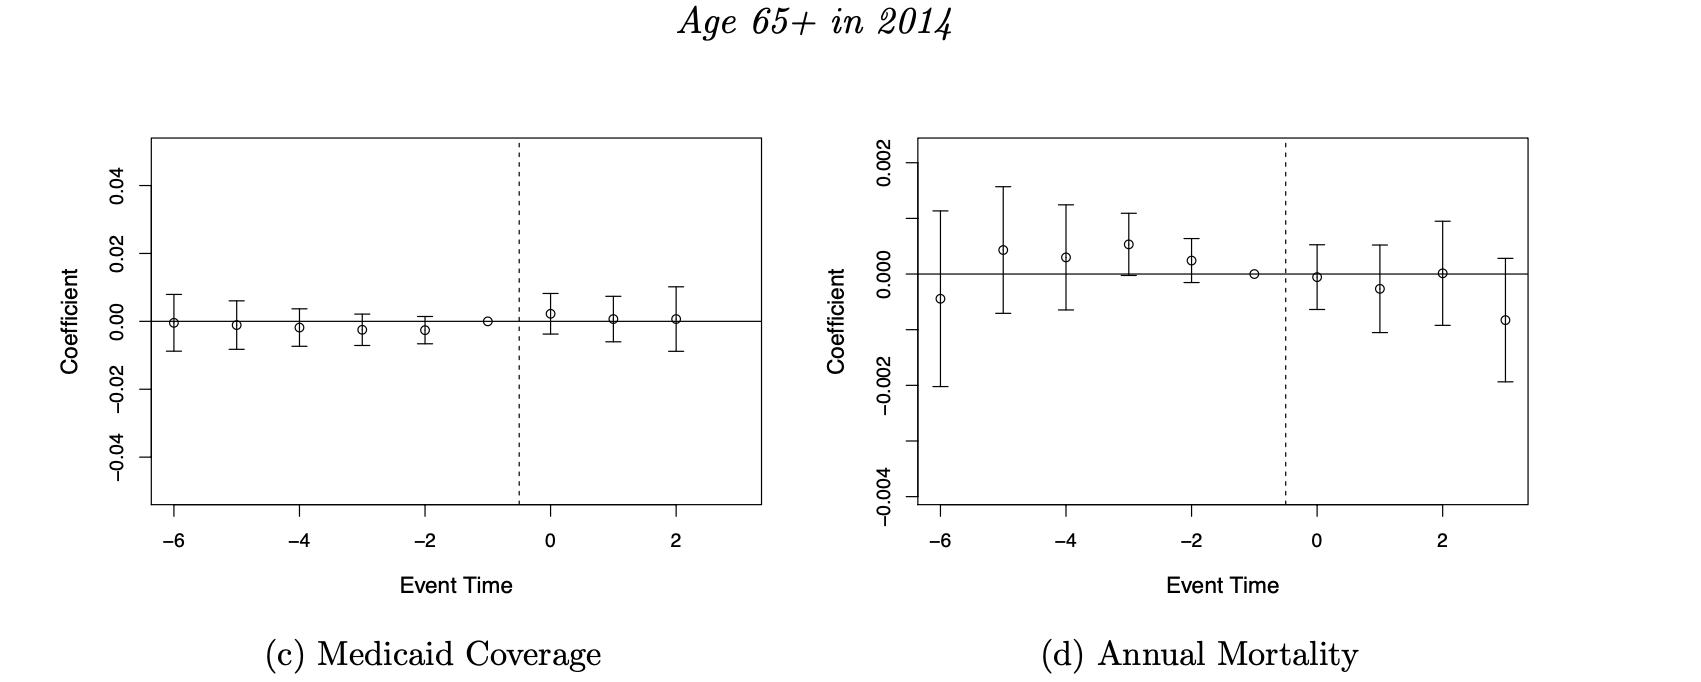
\includegraphics[scale=0.425]{./lecture_includes/placebo_medicaid}
	\end{figure}

\end{frame}



\begin{frame}[plain]

	\begin{figure}
	\includegraphics[scale=0.3]{./lecture_includes/Miller_Medicaid4.png}
	\caption{Miller, et al. (2019) estimates of Medicaid expansion's effects on on annual mortality}
	\end{figure}

\end{frame}

\begin{frame}{Mechanism}

\begin{itemize}
\item Bite: Increases in enrollment and reductions in uninsured support that there is adoption of the treatment
\item Main Results: 9.2\% reduction in mortality among the near-elderly
\item Falsifications: no effect on a similar group who isn't eligible
\item Mechanism: ``The effect is driven by a reduction in disease-related deaths and grows over time.''
\item Event studies: Compelling once the others are established
\end{itemize}

\end{frame}

\begin{frame}{Making event study}

\begin{itemize}
\item All the simple event study is is an interaction between the treatment group dummy and the calendar year dummies
\item You must drop a $t-\tau$ as the baseline (e.g., $t-1$) must be $Y^0$ untreated comparisons recall
\item I have included in a do file that will do it for you either manually or using coefplot in \texttt{simple\_eventstudy.do} at github labs
\end{itemize}

\end{frame}


\begin{frame}{Manually creating the event study}

	\begin{figure}
	\includegraphics[scale=0.20]{./lecture_includes/simple_eventstudy_manual}
	\end{figure}

\end{frame}




\begin{frame}{Creating the event study with Ben Jann's \texttt{coefplot}}

	\begin{figure}
	\includegraphics[scale=0.20]{./lecture_includes/simple_eventstudy.png}
	\end{figure}

\end{frame}





\subsection{Falsifications}


\begin{frame}{Falsifications on more comparison groups}
	
	\begin{itemize}
	\item Very common for readers and others to request a variety of ``robustness checks'' from a DD design
	\item We saw some of these just now (e.g., falsification test using data for alternative control group, the Medicare population)
	\item Triple differences is another way to do that, but it will have a somewhat different parallel trends assumption
	\end{itemize}
\end{frame}





\begin{frame}{Biased diff-in-diff \#1}

\begin{table}\centering
\scriptsize
		\caption{Biased diff-in-diff \#1: comparing states}
		\begin{center}
		\begin{tabular}{lll|lc}
		\toprule
		\multicolumn{1}{l}{\textbf{States}}&
		\multicolumn{1}{c}{\textbf{Period}}&
		\multicolumn{1}{c}{\textbf{Outcomes}}&
		\multicolumn{1}{c}{$D_1$}&
		\multicolumn{1}{c}{$D_2$}\\
		\midrule
		Experimental states & Before & $Y=NJ$ \\
		& After & $Y=NJ + NJ_t + D$ & $\textcolor{red}{NJ_t}+D$\\
		\midrule
		& & & & $D + (\textcolor{red}{NJ_t}- PA_t)$ \\
		\midrule
		Non-experimental  & Before & $Y=PA$ \\
		states& After & $Y=PA + PA_t$ & $PA_t$\\
		\bottomrule
		\end{tabular}
		\end{center}
	\end{table}

\begin{eqnarray*}
\widehat{\delta}_{did} = D + (\textcolor{red}{NJ_t}- PA_t)
\end{eqnarray*}The ATT is D. Diff-in-diff is an unbiased estimate of D if $\textcolor{red}{NJ_t} = PA_t$. Call parallel trends.

\end{frame}


\begin{frame}{Biased diff-in-diff \#2}

\begin{table}\centering
\scriptsize
		\caption{Biased diff-in-diff \#2: comparing groups}
		\begin{center}
		\begin{tabular}{lll|lc}
		\toprule
		\multicolumn{1}{l}{\textbf{Groups}}&
		\multicolumn{1}{c}{\textbf{Period}}&
		\multicolumn{1}{c}{\textbf{Outcomes}}&
		\multicolumn{1}{c}{$D_1$}&
		\multicolumn{1}{c}{$D_2$}\\
		\midrule
		Married women & Before & $Y=MW$ \\
		& After & $Y=MW + MW_t + D$ & $\textcolor{red}{MW_t}+D$\\
		\midrule
		& & & & $D + (\textcolor{red}{MW_t}- SO_t)$ \\
		\midrule
		Single men  & Before & $Y=SO$ \\
		and older women& After & $Y=SO + SO_t$ & $SO_t$\\
		\bottomrule
		\end{tabular}
		\end{center}
	\end{table}

\begin{eqnarray*}
\widehat{\delta}_{did} = D + (\textcolor{red}{MW_t}- SO_t)
\end{eqnarray*}Also unbiased estimate of D if $\textcolor{red}{MW_t} = SO_t$. A different parallel trends assumption.

\end{frame}


\begin{frame}{Two biased diff-in-diffs}

\begin{itemize}

\item If parallel trends of one doesn't hold, use the other, because both identify the ATT under their respective parallel trends
\item But what if both of them are biased -- then you can't use diff-in-diff because diff-in-diff requires at least one parallel trends
\item Okay, but what if both biases are the same?
	\begin{eqnarray*}
	(\textcolor{red}{NJ_t} -PA_t) = (\textcolor{red}{MW_t} - SO_t)
	\end{eqnarray*}
\item Then you can use triple differences, first developed by Gruber (1994)

\end{itemize}

\end{frame}

\begin{frame}{Triple differences by Gruber (1995)}
	
	\begin{figure}
	\includegraphics{./lecture_includes/gruber_ddd_3.pdf}
	\end{figure}
	
\end{frame}

\begin{frame}{Triple differences commentary}

\begin{itemize}

\item In Gruber's 1994 article, it isn't clear why he needed triple differences in the first place -- his triple differences yielded -0.054 which is almost the same as what he found with his first diff-in-diff (-0.062)
\item The main value of triple differences is that you use it when you believe the parallel trends assumption doesn't hold

\end{itemize}

\end{frame}


\begin{frame}[shrink=20]

\begin{table}\centering
		\caption{Difference-in-Difference-in-Differences (Gruber version)}
		\tiny
		\begin{center}
		\begin{tabular}{lll|l|lll}
		\toprule
		\multicolumn{1}{l}{\textbf{Groups}}&
		\multicolumn{1}{c}{\textbf{States}}&
		\multicolumn{1}{c}{\textbf{Period}}&
		\multicolumn{1}{c}{\textbf{Outcomes}}&
		\multicolumn{1}{c}{$D_1$}&
		\multicolumn{1}{c}{$D_2$}&
		\multicolumn{1}{c}{$D_3$}\\
		\midrule
		&&After	&$NJ+MW+\textcolor{blue}{NJ_t}+\textcolor{red}{MW_t}+D$					\\
	&Experimental			&&&$\textcolor{blue}{NJ_t}+MW_t + D$			\\
		&states&Before	&$NJ+MW$					\\
Married women 					&&&&&$D+\textcolor{blue}{NJ_t} -PA_t 	$	\\
20-40							&&&&&$$\\
    		&&After	&$PA+MW+PA_t+MW_t$					\\
	&Non-experimental		&&	&$PA_t+MW_t$				\\
		&states&Before	&$PA+MW$					\\
								\\
&&&&&&$\textcolor{black}{D}$
\\
		&&After	&$NJ+SO+NJ_t+SO_t$				\\
	&Experimental 			&&&$NJ_t+SO_t$ \\				
		&states&Before	&$NJ+SO$					\\
Single men 					&&&&&$NJ_t  - PA_t$		\\
Older women					&&&&&$$		\\
	     	&&After	&$PA+SO+PA_t+SO_t$					\\
	&Non-experimental		&&&	$PA_t+SO_t$				\\
		&states&Before	&$PA+SO$					\\
		\bottomrule
		\end{tabular}
		\end{center}
	\end{table}

\begin{center}
\textbf{Triple diff assumption}
\end{center}

$\widehat{\delta}_{DDD}= D + \underbrace{[(\textcolor{blue}{NJ^{MW}_t} - PA^{MW}_t) -( NJ^{SO}_t - PA^{SO}_t )]}_{\mathclap{\text{Equally biased  DiD \#1 and \# 2}}}$

\bigskip
Triple differences requires two diff-in-diff, from different groups, with the same bias. Parallel bias


\end{frame}







\begin{frame}{DDD in Regression}
	
	\begin{eqnarray*}
	Y_{ijt} &=&\alpha +  \beta_2 \tau_t + \beta_3 \delta_j  + \beta_4 D_i + \beta_5(\delta \times \tau)_{jt} \\
	&& +\ \beta_6(\tau \times D)_{ti} +  \beta_7(\delta \times D)_{ij} +  \textcolor{red}{\beta_8(\delta \times \tau \times  D)_{ijt}}+  \varepsilon_{ijt}
	\end{eqnarray*}
	
	\begin{itemize}
	\item Your panel is now a group $j$ state $i$ (e.g., AR high wage worker 1991, AR high wage worker 1992, etc.)
	\item Assume we drop $\tau_t$ but I just want to show it to you for now.
	\item If the placebo DD is non-zero, it might be difficult to convince the reviewer that the DDD removed all the bias 
	\end{itemize}
	
\end{frame}

\begin{frame}{Great new paper to learn more}

\begin{figure}
\includegraphics[scale=0.25]{./lecture_includes/olden_moen_2022_ddd.png}
\end{figure}

\end{frame}




\begin{frame}{Falsification on outcomes}
	
	\begin{itemize}
	\item The within-group control group (DDD) is a form of placebo analysis using the same \emph{outcome}
	\item But there are also placebos using a \emph{different} outcome -- but you need a hypothesis of mechanisms to figure out what is in fact a \emph{different outcome}
	\item Figure out what those are, and test them -- finding no effect on placebo outcomes tends to help people your other results interestingly enough
	\item Cheng and Hoekstra (2013) examine the effect of castle doctrine gun laws on non-gun related offenses like grand theft auto and find no evidence of an effect 
	\end{itemize}
\end{frame}



\begin{frame}{Rational addiction as a placebo critique}


Sometimes, an empirical literature may be criticized using nothing more than placebo analysis

\begin{quote}``A majority of [our] respondents believe the literature is a success story that demonstrates the power of economic reasoning.  At the same time, they also believe the empirical evidence is weak, and they disagree both on the type of evidence that would validate the theory and the policy implications. Taken together, this points to an interesting gap.  On the one hand, most of the respondents claim that the theory has valuable real world implications.  On the other hand, they do not believe the theory has received empirical support.''
\end{quote}

\end{frame}

\begin{frame}{Placebo as critique of empirical rational addiction}

\begin{itemize}
	\item Auld and Grootendorst (2004) estimated standard ``rational addiction'' models (Becker and Murphy 1988) on data with milk, eggs, oranges and apples.  
	\item They find these plausibly non-addictive goods are addictive, which casts doubt on the empirical rational addiction models.
\end{itemize}

\end{frame}

\begin{frame}{Placebo as critique of peer effects}

\begin{itemize}
	\item Several studies found evidence for ``peer effects'' involving inter-peer transmission of smoking, alcohol use and happiness tendencies
	\item Christakis and Fowler (2007) found significant network effects on outcomes like obesity
	\item Cohen-Cole and Fletcher (2008) use similar models and data and find similar network ``effects'' for things that \emph{aren't} contagious like acne, height and headaches
	\item Ockham's razor - given social interaction endogeneity (Manski 1993), homophily more likely explanation
\end{itemize}

\end{frame}

\section{Interesting Applications using staggered adoption}

\subsection{Facebook and Mental Health}

\begin{frame}{Bringing them together}

\begin{itemize}

\item An advanced area is when areas adopt policies at different points in time -- called differential timing
\item Very popular, but methodologically somewhat more complex than the one we've reviewed
\item I'm going to just walk you through their findings, and if you're interested in learning more about this, then you can attend my workshop for \$1 in a few weeks!

\end{itemize}

\end{frame}


\begin{frame}
\begin{center}
\includegraphics[scale=0.35]{./lecture_includes/facebook_quote}
\end{center}
\end{frame}



\begin{frame}{Mental health and Social Media}

\begin{itemize}
\item Unclear what he means; he may mean there is no experimental evidence
\item Very difficult to imagine a randomized experiment -- especially once the claim out there is that it is harmful, Institutional Review Boards likely wouldn't approve it
\item Quasi-experimental evidence can step in to answer important questions like this
\item Braghieri, Levy and Makarin (2022), ``Social Media and Mental Health'', \emph{American Economic Review}, 112(11): 3660-3693


\end{itemize}

\end{frame}

\begin{frame}{Overview of design and data}

\begin{itemize}
\item Authors take advantage of a clever quirk in Facebook (then ``theFacebook'') targeted different universities from 2004 to 2006
\item They found an online data source that allowed them to pin point precisely when a university was ``treated'' with theFacebook
\item They then linked that data with a longrunning health survey of college students (both before and after) in a very clever way
\item Estimated the effect of a new social media platform's presence at a university on student revealed mental health problems

\end{itemize}

\end{frame}


\begin{frame}{DID in Court}

Five elements of a strong DiD
\begin{enumerate}

\item \textbf{Bite}: \textcolor{red}{Nothing}. They cannot really show much here.  No data on Facebook usage.  They had to rely on anecdote and Facebook as a ``first mover'', but there had been Friendster and MySpace so this does weaken the paper maybe
\item \textbf{Main Results}: Very strong evidence, mostly expressed using rich survey data and questions transformed into z-scores (standard deviations)
\item \textbf{Falsifications}: \textcolor{red}{None}. Authors do not perform falsifications. Remember Miller, Johnson and Wherry looking at Medicaid's effect on Medicare eligible population?  There isn't anything like that here.
\item \textbf{Event studies}: Extremely compelling evidence and robustness across a half dozen different models
\item \textbf{Mechanism}: \textcolor{red}{Very weak in my opinion}

\end{enumerate}

\end{frame}

\begin{frame}{DiD in Court}

\begin{itemize}

\item So in many ways the strength of the project lies in a few areas:
	\begin{enumerate}
	\item Important question -- social media and youth mental health problems is a major policy question (see Zuckerberg testifying before Congress about it)
	\item Excellent research design -- difference-in-differences
	\item Meticulous data collection
	\item Data visualization is compelling
	\end{enumerate}
\item And it publishes in the premiere journal in economics, which I think shows that the research question and high quality data combined with research design can lift a paper

\end{itemize}

\end{frame}







\begin{frame}{TWFE}

\begin{equation}
Y_{icgt} = \alpha_g + \delta_t + \beta \times Facebook_{gt} + X_i \times \gamma + X_c \times \psi + \varepsilon_{icgt}
\end{equation}

\bigskip

This is a version of the regression model we looked at called "twoway fixed effects".  Somewhat complicated to dig into, so I will just say that they use it plus some other methods that are appropriate when you have several difference-in-differences events.  But the focus is on $\beta$

\end{frame}


\begin{frame}{Data on Facebook}

\begin{itemize}

\item When does Facebook appear at a school?  
	\begin{itemize}
	\item Facebook only publishes a fraction of that information
	\item They came up with a workaround
	\end{itemize}
\item The Wayback Machine has been taking almost daily photographs of every website since the Internet's beginning -- including the frontpage of ``TheFacebook''
\item Guess what was on the front page of TheFacebook \dots

\end{itemize}

\end{frame}

\begin{frame}
\begin{center}
\includegraphics[scale=0.25]{./lecture_includes/wayback1}
\end{center}
\end{frame}

\begin{frame}
\begin{center}
\includegraphics[scale=0.35]{./lecture_includes/wayback2}
\end{center}
\end{frame}

\begin{frame}
\begin{center}
\includegraphics[scale=0.25]{./lecture_includes/wayback3}
\end{center}
\end{frame}

\begin{frame}
\begin{center}
\includegraphics[scale=0.25]{./lecture_includes/wayback4}
\end{center}
\end{frame}

\begin{frame}{Timing Dates}

\begin{itemize}
\item They went through three years of daily screenshots on Wayback machine to find when a school appeared on the front page
\item The first time Agnes Scott, or Covenant, appears on the front page, the authors mark that as the date when the school got Facebook
\item But now they need information on mental health outcomes
\item They find it with an old long running repeated cross section survey of college students
\end{itemize}

\end{frame}

\begin{frame}{NCHA survey by ACHA}

\begin{quote}
Our second main data source consists of more than 430,000 responses to the NCHA survey, a survey administered to college students on a semi-annual basis by the American College Health Association (ACHA). The NCHA survey was developed in 1998 by a team of college health professionals with the purpose of obtaining information from college students about their mental and physical health. Specifically, the NCHA survey inquires about demographics, physical health, \textbf{mental health}, alcohol and drug use, sexual behaviors, and perceptions of these behaviors among one’s peers.
\end{quote}

\end{frame}

\begin{frame}{No evidence of bite}

\begin{quote}
The NCHA survey does not include any questions on social media use; therefore, it is not possible for us to determine whether a particular survey respondent had a Facebook account.
\end{quote}

\bigskip

This is probably the problem in any study in which your treatment is more or less the first of its kind -- most likely the standard surveys have not yet incorporated the questions into their surveys

\end{frame}

\begin{frame}{Linking Facebook data with NCHA data}

\begin{quote}
In order to protect the privacy of the institutions that participate in the NCHA survey while still allowing us to carry out the analysis, the ACHA kindly agreed to provide us with a customized dataset that includes a variable indicating the semester in which Facebook was rolled out at each college. Specifically, the ACHA adopted the following procedure: (i) merge our dataset containing the Facebook introduction dates to the NCHA dataset; (ii) add a variable listing the semester in which Facebook was rolled out at each college;15 (iii) strip away any information that could allow us to identify colleges (including the specific date in which Facebook was introduced at each college).
\end{quote}

\end{frame}

\begin{frame}{Basic facts about early and late adopters}

\begin{itemize}
\item Colleges in earlier Facebook expansion groups are more selective in terms of test scores, larger, more likely to be on the East Coast, and have more residential undergraduate programs than colleges in later Facebook expansion groups. 

\item Colleges in earlier Facebook expansion groups enroll students from relatively more advantaged economic backgrounds. 

\item Students in colleges that received Facebook relatively earlier have worse baseline mental health outcomes than students attending colleges in later Facebook expansion groups. 

%The baseline differences across Facebook expansion groups may lead one to wonder about the plausibility of the parallel trends assumption in this setting; we address concerns related to parallel trends in Section III.

\end{itemize}

\end{frame}

\begin{frame}{Measurement}

\begin{itemize}
\item The survey data is very rich with a lot of questions about mental health with different scales
\item They create their own combinations of these questions into aggregate indices -- ``index of poor mental health'' where higher numbers mean worse mental health
\item Each outcome survey question is normalized into what is called a ``z-score'' which is interpreted as a fraction of a standard deviation
\item Estimates are ATT parameters -- average effect of Facebook on students at schools that got Facebook
\end{itemize}

\end{frame}


\begin{frame}
\begin{center}
\includegraphics[scale=0.35]{./lecture_includes/facebook_1}
\end{center}
\end{frame}

\begin{frame}
\begin{center}
\includegraphics[scale=0.35]{./lecture_includes/facebook_2}
\end{center}
\end{frame}

\begin{frame}
\begin{center}
\includegraphics[scale=0.35]{./lecture_includes/facebook_3}
\end{center}
\end{frame}

\begin{frame}
\begin{center}
\includegraphics[scale=0.35]{./lecture_includes/facebook_4}
\end{center}
\end{frame}

\begin{frame}
\begin{center}
\includegraphics[scale=0.35]{./lecture_includes/facebook_5}
\end{center}
\end{frame}

\begin{frame}
\begin{center}
\includegraphics[scale=0.35]{./lecture_includes/facebook_6}
\end{center}
\end{frame}

\begin{frame}
\begin{center}
\includegraphics[scale=0.35]{./lecture_includes/facebook_7}
\end{center}
\end{frame}

\begin{frame}{Questions and Comments}

\begin{itemize}
\item Mark Zuckerberg quote: ``the existing body of scientific work has not shown a causal link between using social media and young people having worse mental health outcomes'' -- What is your reaction to his claim?
\item What is your reaction to this study's evidence?  
\item Which parts of this study do you think is more memorable and more convincing and why?
\item How might you replicate this study yourself?

\end{itemize}

\end{frame}

\subsection{Generative AI Randomized Experiment}

\begin{frame}{Generative AI and Workers}
\begin{itemize}
  \item Generative AI systems create content that mimics human creativity across various media.
  \item May have large impacts on some kinds of jobs, but unclear to what degree and how soon
  \item Unclear whether we should be concerned, and we can't devise a lot of policies if we don't understand what effects might be
\end{itemize}
\end{frame}


\begin{frame}{What is a Large Language Model?}
\begin{itemize}
  \item Large Language Models (LLMs) like ChatGPT3, 3.5 and 4 are at the forefront of this change.
  \item LLMs learn from (``train on'') large datasets of writings to produce human-like language.
  \item Think of it like autocorrect on your phone, only it's generating entire conversations, not just the next letter or word
  \item These models power diverse applications, from chatbots to data analysis tools.
\end{itemize}
\end{frame}


\begin{frame}{The Evolution of OpenAI}
\begin{itemize}
  \item OpenAI was founded in 2015 by Sam Altman, Elon Musk, Greg Brockman, and several others as a non-profit  aimed to ensure artificial intelligence benefits all of humanity, marking a commitment to openness and safety in AI development.
  \item Initially, OpenAI focused on reinforcement learning and unsupervised learning but quickly adapted to the transformative potential of transformers after 2017 when Google published a paper entitled ``Attention is All You Need'' introducing transformer models
  \item The organization's pivot towards transformer-based models like GPT was driven by the architecture's ability to process and generate natural language more effectively than previous models.
\end{itemize}
\end{frame}



\begin{frame}{Transformers and Generative AI}
\begin{itemize}
  \item The introduction of the transformer model in the "Attention Is All You Need" paper represented a paradigm shift in AI, leading to the development of more advanced and efficient language models.
  \item OpenAI capitalized on this breakthrough, leading to the creation of the Generative Pretrained Transformer series, which significantly advanced the field of natural language processing.
  \item Quickly they realized that the more data they fed these models, the better they got -- nonlinear, not linear, so they invested heavily in computing powers (billions of dollars raised, Microsoft partnership)
\end{itemize}
\end{frame}

\begin{frame}{OpenAI's Response and Innovations Post-2017}
\begin{itemize}
  \item OpenAI's strategic shift to transformers culminated in the release of GPT, GPT-2, and the groundbreaking GPT-3, each setting new benchmarks for AI's capability in understanding and generating human-like text.
  \item The development and release of these models not only showcased OpenAI's leadership in AI research but also underscored the potential of large language models in various applications.
\end{itemize}
\end{frame}

\begin{frame}{The Growth of OpenAI}
\begin{itemize}
  \item OpenAI's journey from a non-profit organization to the creation of a capped-profit arm in 2019 allowed it to attract significant investment and scale its operations, while still adhering to its mission.
  \item The subsequent development and launch of GPT-3.5 and GPT-4 illustrated not only technological advancements but also a significant increase in user adoption and commercial success.
\end{itemize}
\end{frame}

\begin{frame}{Impact and Future Directions}
\begin{itemize}
	\item Exciting time in many ways, but also worrisome
	\item Technologies have always reallocated work -- think of the old horse and buggy industry being replaced by vehicles 
	\item But these technologies may be impacting high skill work which would make it different from the Industrial Revolution
	\item Two causal studies (one experiment and one diff-in-diff) are going to examine this
\end{itemize}
\end{frame}


\begin{frame}{Two studies}

\begin{itemize}

\item First is a randomized controlled trial (RCT) in which ChatGPT-4 was randomly assigned to consultants at Boston Consulting Group to examine  effects on various performance measures
\item Second is a diff-in-diff when a firm rolled out its own generative AI chatbot to assist customer service representatives
\item In both we are trying to understand the impact this had on worker productivity, but we will ask ourselves in the end what we might expect to happen to demand too
\end{itemize}

\end{frame}


\begin{frame}{Study 1: the RCT}

\begin{itemize}

\item Professors at Penn, Harvard and MIT worked with Boston Consulting Group, a global management consulting firm, to examine the performance implications of ChatGPT-4 on realistic, complex and knowledge-intensive tasks
\item Experiment was registered ahead of time and involved 758 consultants comprising 7\% of the individual consultants at the company
\item They then created a realistic, yet fictional, sneaker client and observed consultants' performance on tasks afterwards
\end{itemize}

\end{frame}

\begin{frame}{Design}

Each consultants' baseline skill on tasks was measured and then each was randomized to one of the three following "treatment" conditions

	\begin{enumerate}
	\item No AI access
	\item ChatGPT-4 AI access
	\item ChatGPT-4 access with prompt engineering overview
	\end{enumerate}

\end{frame}

\begin{frame}{Two types of tasks}

\begin{itemize}

\item We tested two distinct tasks: one situated outside the frontier of AI capabilities and the other within its bounds. 
\item The experiment aimed to understand how AI integration might reshape the traditional workflows of these high human capital professionals.

\end{itemize}

\end{frame}


\begin{frame}{Findings}

\begin{quote}

Our results show that this generation of LLMs are highly capable of causing significant increases in quality and productivity, or even completely automating some tasks, but the actual tasks that AI can do are surprising and not immediately obvious to individuals or even to producers of LLMs themselves. Because this frontier is expanding and changing, the overall results suggest that AI will have a large impact on work, one which will increase with LLM capabilities, but where the impacts occur will be uneven.
\end{quote}

\end{frame}


\begin{frame}{Inside the Frontier Tasks}
\begin{center}
\includegraphics[scale=0.35]{./lecture_includes/ethan1}
\end{center}
\end{frame}


\begin{frame}{Inside the Frontier Tasks}
\begin{center}
\includegraphics[scale=0.35]{./lecture_includes/ethan2}
\end{center}
\end{frame}

\begin{frame}{Outside the Frontier Tasks}

\begin{itemize}

\item But a number of things in the study workers treated with ChatGPT-4 performed worse than the control group
\item For those ``outside the frontier'' tasks, consultants using ChatGPT-4 were 19 percentage points less likely to produce correct solutions compared to control group

\end{itemize}

\end{frame}

\begin{frame}{Summary}

\begin{itemize}

\item So we have some workers -- particularly the least skilled -- becoming just as productive with ChatGPT-4 as the most skilled worker without it
\item But not all types of work does AI help with -- basic math, interestingly, it cannot help with; but for the creation of new ideas, and creative work more generally, for some reason it seems have some improvements
\item That was an RCT with skilled workers -- let's now move to a DiD with a generative AI chatbot rolled out to all of the workers over time

\end{itemize}

\end{frame}


\subsection{ChatBot Rollout}

\begin{frame}{Working Paper on ChatBot}
\begin{center}
\includegraphics[scale=0.35]{./lecture_includes/brynn}
\end{center}
\end{frame}



\begin{frame}{Chatbots and Workers}

\begin{itemize}

\item An unnamed firm released gradually a generative AI-based conversational assistant chatbot to its  5,179 customer support agents 
\item These chatbots provided assistance in handling complaints
\item Very stressful job as the only time customers reached out was when they were very upset
\item It isn't a randomized experiment so they're going to estimate the effect of the adoption of the chatbot using difference-in-differences

\end{itemize}

\end{frame}

\begin{frame}{Outcomes and Pictures}

\begin{itemize}

\item Main focus is on various measures of customer support agents handling of calls, which is the proxy for their productivity
\item But they also focus on high and low skill workers (heterogeneity like before)
\item Authors are going to present evidence almost entirely using event study graphs
\item They also present regression tables, but the event study graphs are very powerful

\end{itemize}

\end{frame}




\begin{frame}{Example of ChatBot}
\begin{center}
\includegraphics[scale=0.35]{./lecture_includes/brynn1}
\end{center}
\end{frame}


\begin{frame}{Rollout}
\begin{center}
\includegraphics[scale=0.35]{./lecture_includes/brynn2}
\end{center}
\end{frame}


\begin{frame}{Resolutions of Customer Problems}
\begin{center}
\includegraphics[scale=0.25]{./lecture_includes/brynn3}
\end{center}
\end{frame}


\begin{frame}{Additional Outcomes}
\begin{center}
\includegraphics[scale=0.35]{./lecture_includes/brynn4}
\end{center}
\end{frame}

\begin{frame}{Heterogeneity by Skill}
\begin{center}
\includegraphics[scale=0.25]{./lecture_includes/brynn5}
\end{center}
\end{frame}


\begin{frame}{Heterogeneity by Skill}
\begin{center}
\includegraphics[scale=0.25]{./lecture_includes/brynn6}
\end{center}
\end{frame}

\begin{frame}{Heterogeneity by Worker Tenure}
\begin{center}
\includegraphics[scale=0.35]{./lecture_includes/brynn7}
\end{center}
\end{frame}



\begin{frame}{Sentiment}
\begin{center}
\includegraphics[scale=0.35]{./lecture_includes/brynn8}
\end{center}
\end{frame}


\begin{frame}{Sentiment}
\begin{center}
\includegraphics[scale=0.3]{./lecture_includes/brynn11}
\end{center}
\end{frame}


\begin{frame}{Manager Assistance}
\begin{center}
\includegraphics[scale=0.25]{./lecture_includes/brynn9}
\end{center}
\end{frame}


\begin{frame}{Outcomes}

\begin{itemize}

\item Across many dimensions, worker productivity rose
\item And the productivity increases were higher for the least skilled workers -- just like we had seen in the experiment
\item They suggest that generative AI ``reallocated experience'' to the least experienced workers making them essentially appear as though they had been their awhile
\item Findings suggest that it improves customer sentiment, reduces requests for managerial intervention, and improves employee retention
\item Still unclear how generalizeable this is, and what impact we should see on overall aggregate employment as this was AI assisted, not AI alone

\end{itemize}

\end{frame}


\section{Conclusion}



\begin{frame}{DiD vs ATT}

\begin{itemize}

\item We learned that difference-in-differences was just four averages and three subtractions
\item But it was also a specific regression specification
\item We saw that difference-in-differences could be used to estimate average treatment effects 
\item But the DiD equation is distinct from the ATT parameter we care about

\end{itemize}

\end{frame}


\begin{frame}{Parallel Trends}

\begin{itemize}

\item DiD only was equal to the ATT if the parallel trends assumption was true
\item But it's not verifiable so it's a difficult assumption
\item Parallel trends is not something a statistical model fixes -- it's something a control group fixes
\item Some comparison groups will satisfy parallel trends, but some won't

\end{itemize}

\end{frame}

\begin{frame}{Evidence for parallel trends}

\begin{enumerate}

\item Event study graphics -- plot coefficients and confidence intervals to check if pre-trends are zero so that post-treatment coefficients are compelling evidence for causal effects
\item Falsifications -- if possible, rule out competing hypotheses using falsifications (e.g., 65+ year olds can't be on Medicaid as they're already on Medicare)

\end{enumerate}

\end{frame}

\begin{frame}{Roadmap}

\begin{enumerate}
\item Show bite -- first order effects
\item Main results -- What's your study about?
\item Event study graphs -- This will be your main results and your evidence of parallel trends keeping in mind pre-trends and parallel trends are technically distinct
\item Falsifications -- If you can find falsifications, use them
\item Mechanisms -- can you find any explanation?
\end{enumerate}

\end{frame}

\begin{frame}{Synthetic control}

\begin{itemize}

\item But what if parallel trends really isn't realistic -- what then?
\item Then you may need to create your own control group that follows the same approximately trajectory as your treatment group pre-treatment
\item A method by Abadie and Gardazebal (2003) and follow up papers worked out a method for this called synthetic control
\item If we have time, we will go through this together

\end{itemize}

\end{frame}






\end{document}


\begin{frame}{Mechanism}

\begin{itemize}

\item Story is interpersonal comparisons which they try to show 
\item We can discuss how plausible we found it, but ask yourself at the end -- did the event study help you believe it?  Why/why not?

\end{itemize}

\end{frame}
